\documentclass[tikz,border=0pt]{standalone}
\usepackage[american]{circuitikz}
\usetikzlibrary{arrows.meta,calc,positioning,decorations.pathmorphing,patterns}
\definecolor{zyloTeal}{HTML}{174A5B}
\definecolor{zyloTealTwo}{HTML}{246B7A}
\definecolor{zyloInk}{HTML}{1F2933}
\definecolor{zyloSoft}{HTML}{EAF4F4}
\definecolor{zyloPaper}{HTML}{F8FAFB}
\definecolor{zyloLine}{HTML}{44606B}
\definecolor{zyloOrange}{HTML}{D97706}
\begin{document}
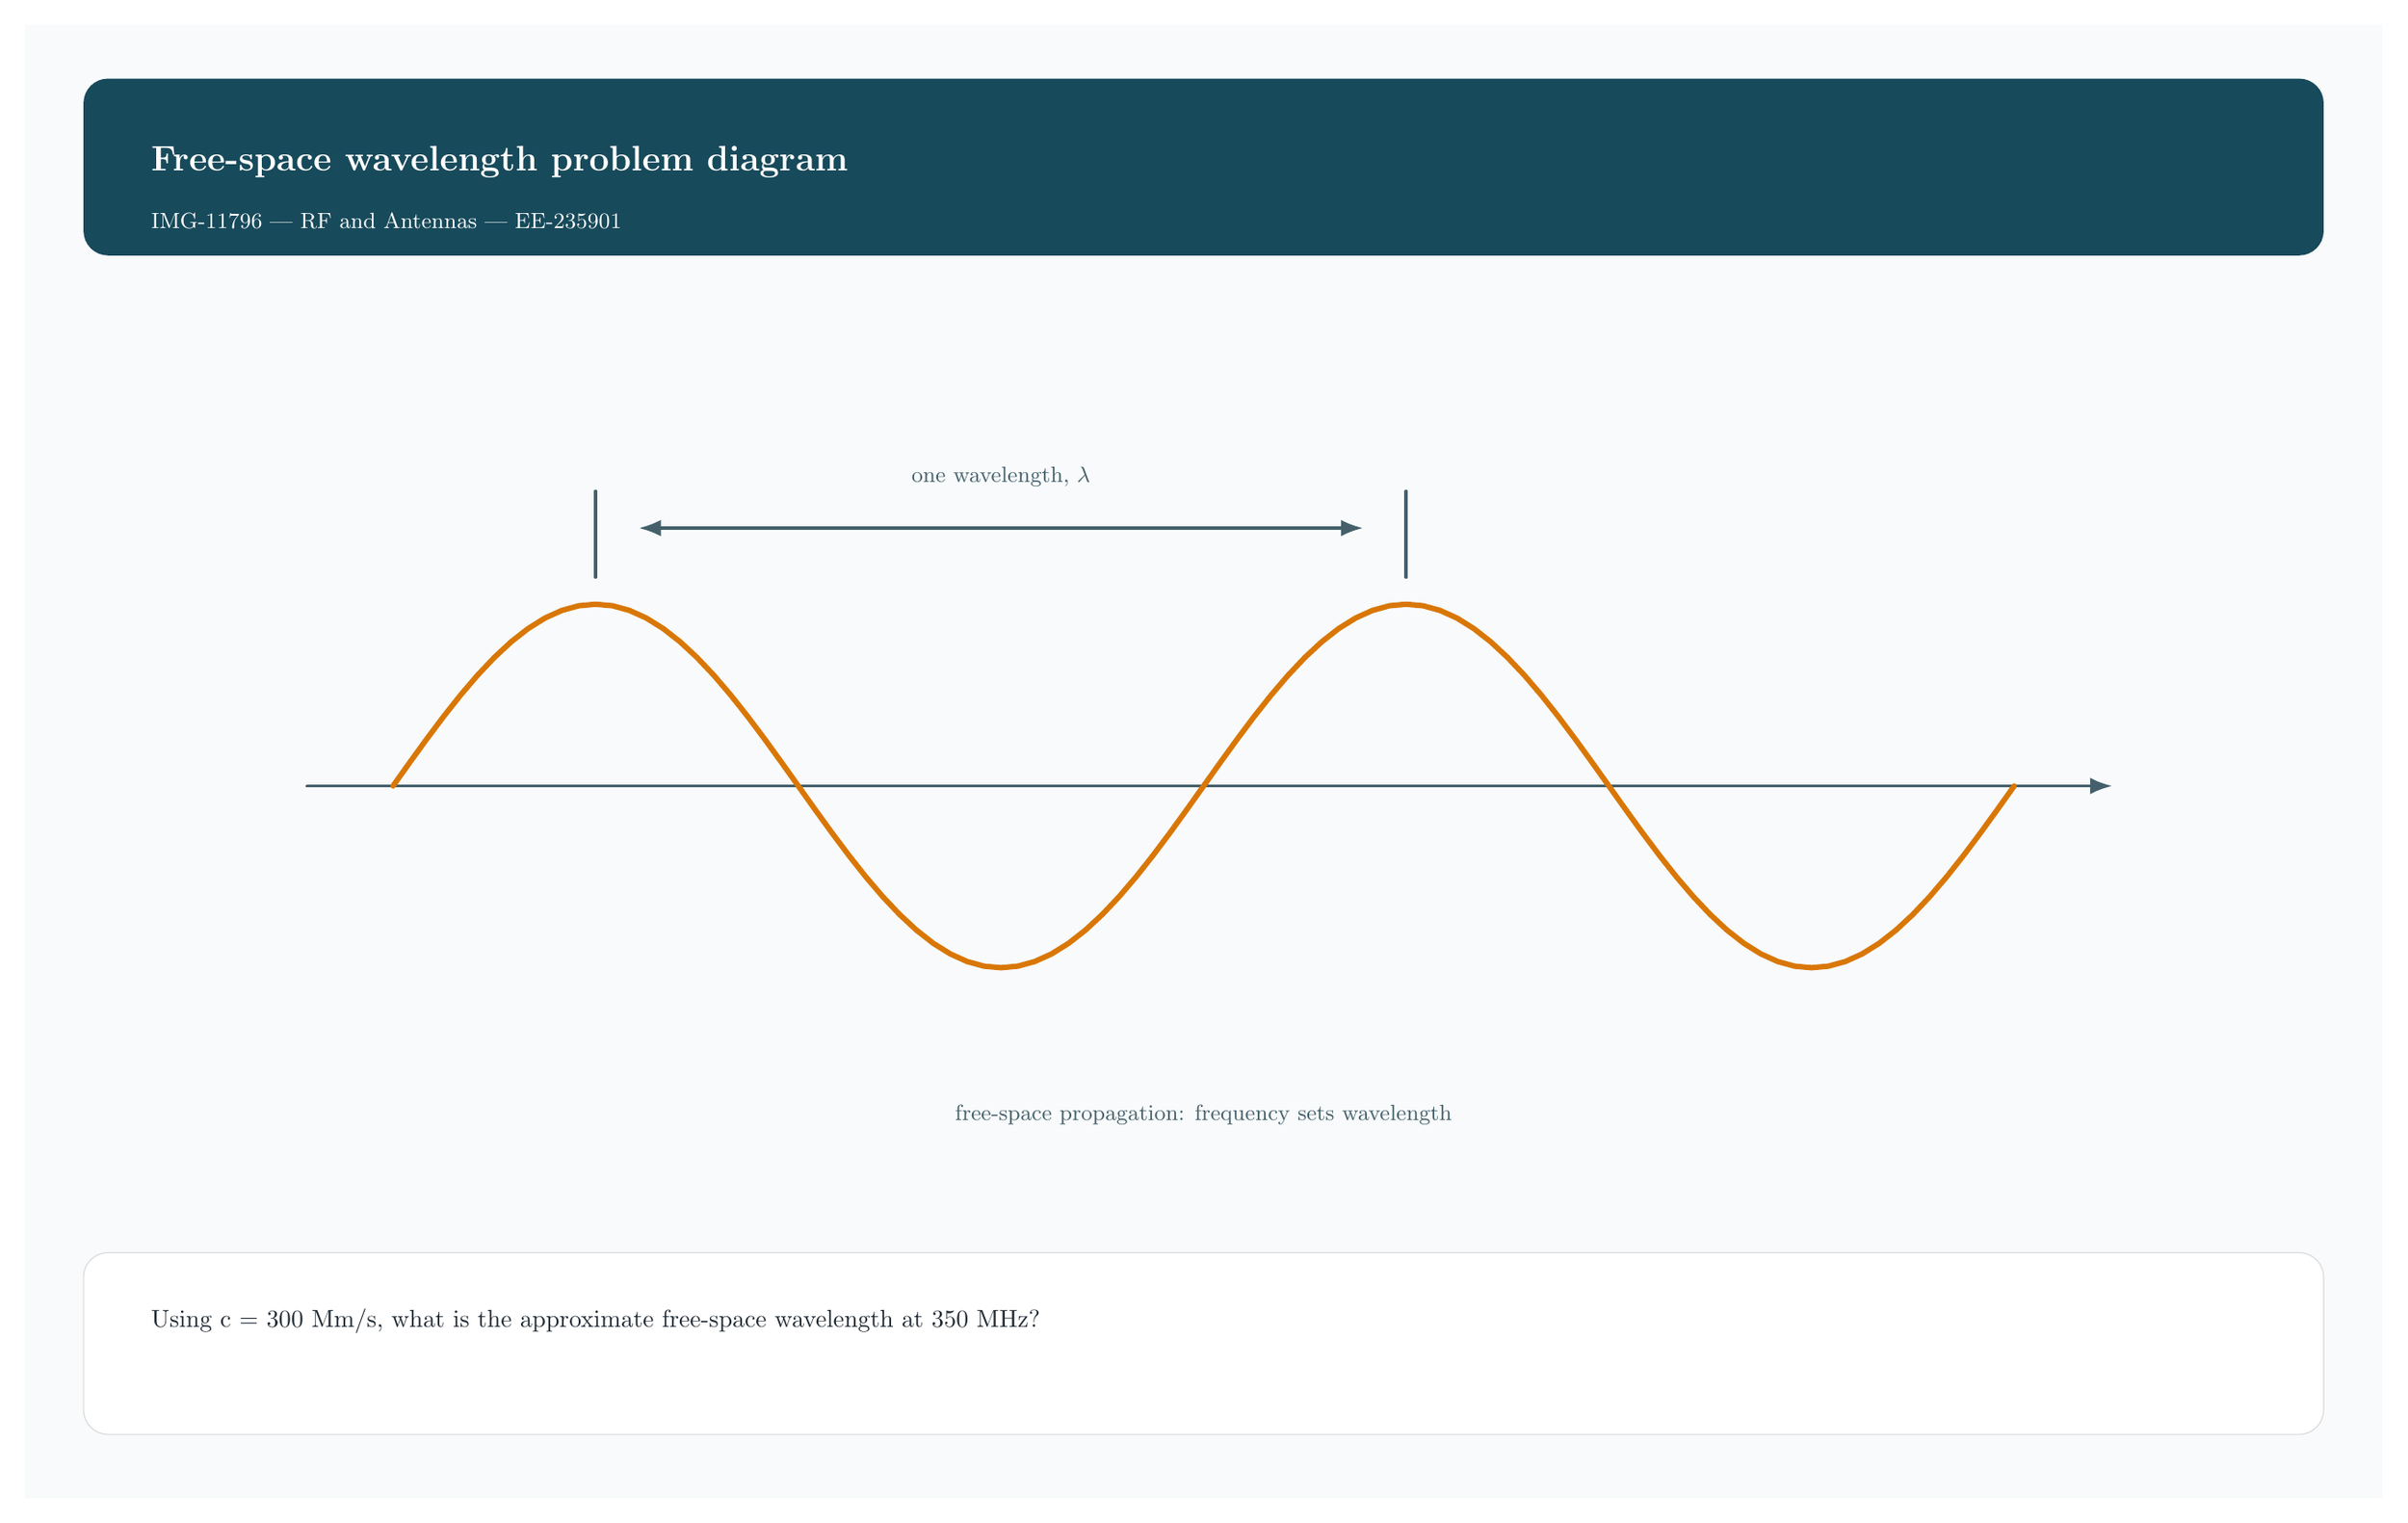
\begin{tikzpicture}[x=1pt,y=-1pt,>=Latex,line cap=round,line join=round]
\path[fill=zyloPaper] (0,0) rectangle (960,600);
\path[fill=zyloTeal,rounded corners=10pt] (24,22) rectangle (936,94);
\node[anchor=west,text=white,font=\bfseries\Large] at (48,56) {Free-space wavelength problem diagram};
\node[anchor=west,text=white!82,font=\small] at (48,80) {IMG-11796 | RF and Antennas | EE-235901};
\tikzset{wire/.style={draw=zyloTeal,line width=2.2pt},thinwire/.style={draw=zyloLine,line width=1.35pt},accent/.style={draw=zyloOrange,line width=2.2pt},box/.style={draw=zyloTealTwo,fill=zyloSoft,line width=1.5pt,rounded corners=8pt}}
\draw[thinwire,->] (115,310) -- (850,310);
\draw[accent] (150,310) -- (156.875,300.341) -- (163.75,290.847) -- (170.625,281.681) -- (177.5,273) -- (184.375,264.952) -- (191.25,257.674) -- (198.125,251.292) -- (205,245.914) -- (211.875,241.633) -- (218.75,238.521) -- (225.625,236.633) -- (232.5,236) -- (239.375,236.633) -- (246.25,238.521) -- (253.125,241.633) -- (260,245.914) -- (266.875,251.292) -- (273.75,257.674) -- (280.625,264.952) -- (287.5,273) -- (294.375,281.681) -- (301.25,290.847) -- (308.125,300.341) -- (315,310) -- (321.875,319.659) -- (328.75,329.153) -- (335.625,338.319) -- (342.5,347) -- (349.375,355.048) -- (356.25,362.326) -- (363.125,368.708) -- (370,374.086) -- (376.875,378.367) -- (383.75,381.479) -- (390.625,383.367) -- (397.5,384) -- (404.375,383.367) -- (411.25,381.479) -- (418.125,378.367) -- (425,374.086) -- (431.875,368.708) -- (438.75,362.326) -- (445.625,355.048) -- (452.5,347) -- (459.375,338.319) -- (466.25,329.153) -- (473.125,319.659) -- (480,310) -- (486.875,300.341) -- (493.75,290.847) -- (500.625,281.681) -- (507.5,273) -- (514.375,264.952) -- (521.25,257.674) -- (528.125,251.292) -- (535,245.914) -- (541.875,241.633) -- (548.75,238.521) -- (555.625,236.633) -- (562.5,236) -- (569.375,236.633) -- (576.25,238.521) -- (583.125,241.633) -- (590,245.914) -- (596.875,251.292) -- (603.75,257.674) -- (610.625,264.952) -- (617.5,273) -- (624.375,281.681) -- (631.25,290.847) -- (638.125,300.341) -- (645,310) -- (651.875,319.659) -- (658.75,329.153) -- (665.625,338.319) -- (672.5,347) -- (679.375,355.048) -- (686.25,362.326) -- (693.125,368.708) -- (700,374.086) -- (706.875,378.367) -- (713.75,381.479) -- (720.625,383.367) -- (727.5,384) -- (734.375,383.367) -- (741.25,381.479) -- (748.125,378.367) -- (755,374.086) -- (761.875,368.708) -- (768.75,362.326) -- (775.625,355.048) -- (782.5,347) -- (789.375,338.319) -- (796.25,329.153) -- (803.125,319.659) -- (810,310);
\draw[thinwire] (232.5,190) -- (232.5,225); \draw[thinwire] (562.5,190) -- (562.5,225); \draw[thinwire,<->] (250,205) -- (545,205);
\node[font=\small,text=zyloLine] at (397.5,184) {one wavelength, $\lambda$};
\node[font=\small,text=zyloLine] at (480,444) {free-space propagation: frequency sets wavelength};
\path[draw=black!15,fill=white,rounded corners=10pt] (24,500) rectangle (936,574);
\node[anchor=west,text width=860pt,align=left,text=zyloInk,font=\normalsize] at (48,528) {Using c = 300 Mm/s, what is the approximate free-space wavelength at 350 MHz?};
\end{tikzpicture}
\end{document}
